\documentclass[12pt]{article}
\usepackage{geometry}
\geometry{margin=5mm}
\usepackage{graphicx}

%Russian-specific packages
%--------------------------------------
\usepackage[T2A]{fontenc}
\usepackage[utf8]{inputenc}
\usepackage[russian]{babel}
%--------------------------------------
 
%Hyphenation rules
%--------------------------------------
\usepackage{hyphenat}
\hyphenation{ма-те-ма-ти-ка вос-ста-нав-ли-вать}
%--------------------------------------

\makeatletter
\renewcommand \dotfill {\leavevmode \cleaders \hb@xt@ 5mm{\hss .\hss }\hfill \kern \z@}
\makeatother

\begin{document}
    \section*{6Н5П}
    \subsection*{Двойной триод с отдельными катодами}
    
    \par
    \begin{minipage}[b][0mm][t]{0.45\textwidth}
        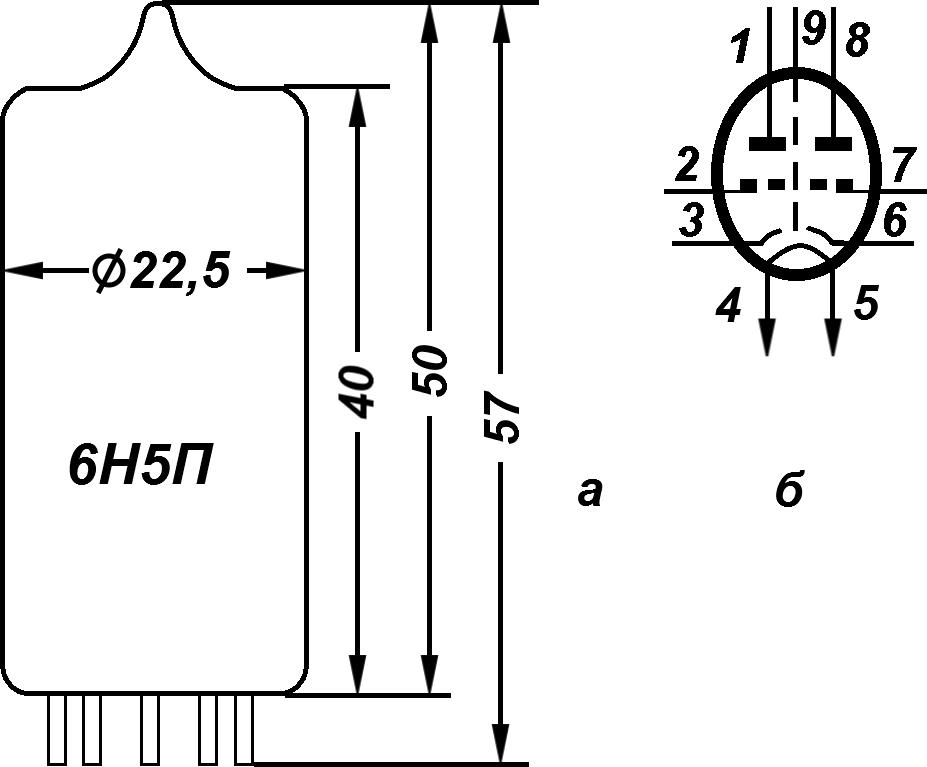
\includegraphics[width=80mm]{symbol.png}
    \end{minipage}
    \begin{minipage}[b][0mm][t]{0.45\textwidth}
        \begin{raggedright}
            \quad Предназначен для усиления напряжения высокой частоты в схемах автоматического регулирования усиления.
            \vspace{2mm}
            \hrule
            \vspace{2mm}
            Рис. 326. Лампа 6Н5П:
            \vspace{-4mm}
            \begin{itemize} \setlength \itemsep{-2.25mm}
                \item[а] --- основные размеры
                \item[б] --- схематическое изображение
                \item[1] --- анод первого триода
                \item[2] --- сетка первого триода
                \item[3] --- катод первого триода
                \item[4 и 5] --- подогреватель (накал)
                \item[6] --- анод второго триода
                \item[7] --- сетка второго триода
                \item[8] --- катод второго триода
                \item[9] --- экран
            \end{itemize}
        \end{raggedright}
    \end{minipage}
    
    \vspace{70mm}
    
    
    \begin{tabular}{l@{}}
        Катод оксидный косвенного накала. \\
        Работает в любом положении. \\
        Выпускается в стеклянном пальчиковом оформлении. \\
        Срок службы не менее 500 ч. \\
        Цоколь 9-штырьковый с пуговичным дном. \\
    \end{tabular}
    
    \vspace{3mm}
    \hspace{-7mm} \textbf{Междуэлектродные емкости, нф}
    \vspace{3mm}
    
    \begin{tabular}{p{105mm}l@{}l}
        Входная каждого триода \hspace{0.1mm} \dotfill & & 3 \\
        Выходная первого триода \dotfill & & 1,5 \\
        Выходная второго триода \dotfill & & 1,7 \\
        Проходная каждого триода \hspace{0.5mm} \dotfill & & 2,25 \\
        Между анодами \hspace{-3.1mm} \dotfill & \hspace{-7mm} не более \hspace{1mm} & 0,2 \\
    \end{tabular}
    
    \vspace{3mm}
    \hspace{-7mm} \textbf{Номинальные электрические данные}
    \vspace{3mm}
    
    \begin{tabular}{p{105mm}l@{}l}
        Напряжение накала, в \hspace{0.1mm} \dotfill & & 6,3 \\
        Напряжение на аноде, в \hspace{-3.1mm} \dotfill & & 200 \\
        Сопротивление в цепи катода для \\
        \hspace{5mm} автоматического смещения, ом \hspace{-2.4mm} \dotfill & & 600 \\
        Ток накала, ма \hspace{-1mm} \dotfill & & 600 $\pm$50 \\
        Ток в цепи анода, ма \hspace{-2.2mm} \dotfill & \hspace{-7mm} не менее \hspace{1mm} & 8 \\
        Крутизна характеристики, ма/в \hspace{-3.4mm} \dotfill & & 4,2 \\
        Коэффициент усиления \hspace{-2.4mm} \dotfill & & 27 \\
    \end{tabular}
    
    \vspace{1mm}
    \hspace{-7mm} \rule{25mm}{0.5mm}
    
    * При запертой лампе (ток в цепи анода 5 мка).
    
    \newpage
    
    \noindent \textbf{Предельно допустимые электрические величины} \\
    (для каждого триода)
    
    \vspace{3mm}
    
    \begin{tabular}{p{105mm}l@{}l}
        Наибольшее напряжение накала, в \hspace{-3.3mm} \dotfill & \hspace{13mm} & 7 \\
        Наименьшее напряжение накала, в \hspace{-3.8mm} \dotfill & & 5,7 \\
        Наибольшее напряжение на аноде, в \dotfill & & 300 \\
        Наибольшая мощность, рассеиваемая \\
        \hspace{5mm} на аноде, вм \hspace{-7.2mm} \dotfill & & 2,2 \\
        Наибольший ток в цепи катода, ма \hspace{-3.9mm} \dotfill & & 25 \\
        Наибольшее постоянное напряжение \\
        \hspace{5mm} между катодом и подогревателем, в \hspace{-7mm} \dotfill & & 250 \\
        Наибольший ток утечки между катодом \\
        \hspace{5mm} и подогревателем, мка \hspace{-6.3mm} \dotfill & & 20 \\
        Наименьшее сопротивление в цепи катода \\
        \hspace{5mm} для автоматического смещения, ом \hspace{-5.5mm} \dotfill & & 600 \\
        Наибольшее сопротивление в цепи сетки, Мом \hspace{-5.5mm} \dotfill & & 1 \\
    \end{tabular}
    
    \vspace{5mm}
    \hspace{-5mm}
    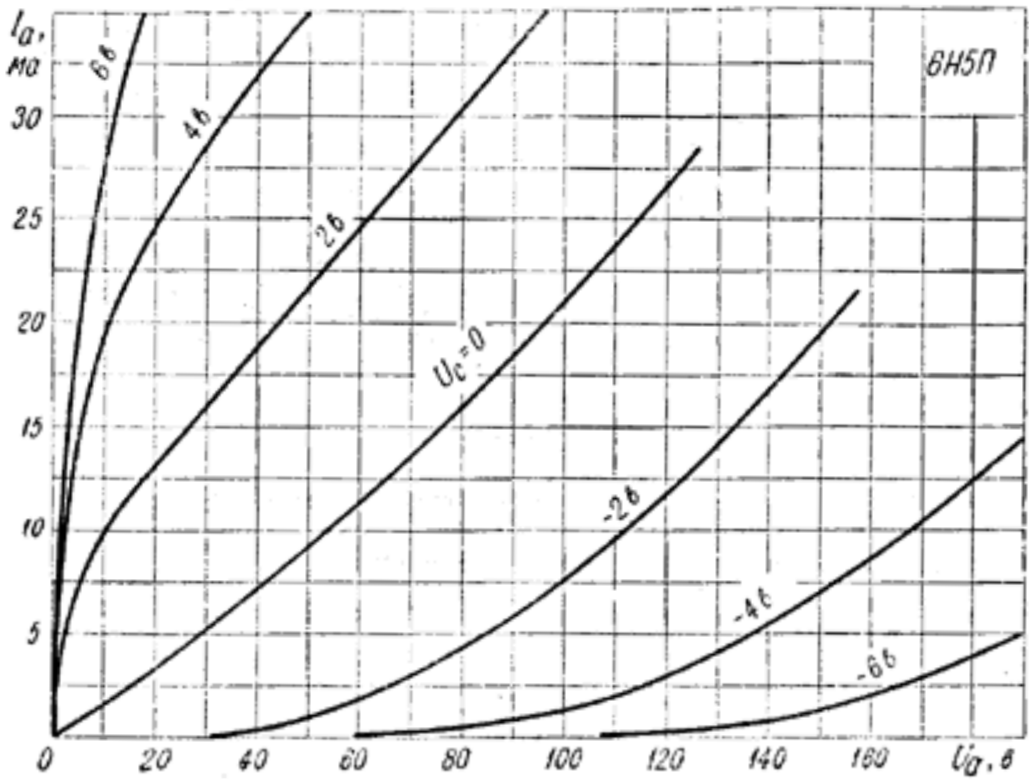
\includegraphics[width=200mm]{graph.png}
    
    Рис. 327, Усредненные характеристики зависимости тока анода от напряжения на аноде.
\end{document}